% !TeX root = Protokoll.tex
\subsection{Bestimmung der Kristallstrukturen}
Für die Bestimmung der Kristallstrukturen müssen die auf die Filmstreifen aufgenommenen Reflexe
mit den nicht verschwindenden Reflexen von kubischen Kristallstrukturen verglichen werden.
Aus der Bragg-Bedingung \eqref{eq:bragg} und der Gleichung \eqref{eq:netzebenen_d} erhält man 
durch Elimination des Netzebenenabstands $d$ und für Reflexe erster Ordnung $n = 1$ die Gleichung
für die Gitterkonstante $a$,
\begin{empheq}{align}
	a &= \frac{\lambda}{2\sin(\theta)}\sqrt{h^2+k^2+l^2}\\
	  \label{eq:gitterkonstante}
	  &= d_{\mathrm{bragg}} \cdot m.
\end{empheq} 
Aus der Konstanz der Gitterkonstante folgt nun, dass für allgemeine Netzebenenabstände $d_{\mathrm{bragg},i}$  und Faktoren $m_i$ 
aus den jeweiligen Millerschen Indizes
\begin{empheq}{equation}
d_{\mathrm{bragg},1} \cdot m_1= d_{\mathrm{bragg},i} \cdot m_i,
\end{empheq} 
folgt. Dabei ist $m_1$ der Faktor für die erste Netzebene mit nicht verschwindenden Reflexen und $d_{\mathrm{bragg},1}$ der 
entsprechende Netzebenenabstand. Daraus ergibt sich die Bedingung, die den Vergleich der aufgenommenen Messwerte mit 
bekannter Kristallstrukturen ermöglicht zu
\begin{empheq}{equation}
  \dfrac{d_{\mathrm{bragg},1}}{d_{\mathrm{bragg},i}}= \dfrac{ m_i}{m_1}.
  \label{eq:bedingung_vergleich}
\end{empheq}

Die Millerschen Indizes der Netzebenen nicht verschwindender Reflexe und der für den Vergleich mit den Messwerten 
benötigte Faktor $\sfrac{m_i}{m_1}$, sind in den Tabellen \ref{tab:reflexe_1_atom} und \ref{tab:reflexe_2_atom} angegeben.
\begin{table}[!h]
	\centering
	\begin{adjustbox}{width=\textwidth}
		\begin{tabular}{cccccccc}
			\toprule
			\multicolumn{2}{c}{einfach}&\multicolumn{2}{c}{flächenzentriert} & \multicolumn{2}{c}{raumzentriert}& \multicolumn{2}{c}{Diamant}\\\cmidrule(rl){1-2}\cmidrule(rl){3-4}\cmidrule(rl){5-6}\cmidrule(rl){7-8}
		Netzebenen & norm. Faktor & Netzebenen & norm. Faktor & Netzebenen & norm. Faktor & Netzebenen & norm. Faktor\\
		$hkl$ & $\frac{m}{m_1}$ & $hkl$ & $\frac{m}{m_1}$ & $hkl$ & $\frac{m}{m_1}$ & $hkl$ & $\frac{m}{m_1}$\\
\midrule
		\num{100} & \num{1.000} & \num{111} & \num{1.000} & \num{110} & \num{1.000} & \num{111} & \num{1.000}\\
		\num{110} & \num{1.414} & \num{200} & \num{1.155} & \num{200} & \num{1.414} & \num{220} & \num{1.633}\\
		\num{111} & \num{1.732} & \num{220} & \num{1.633} & \num{211} & \num{1.732} & \num{311} & \num{1.915}\\
		\num{200} & \num{2.000} & \num{311} & \num{1.915} & \num{220} & \num{2.000} & \num{400} & \num{2.309}\\
		\num{210} & \num{2.236} & \num{222} & \num{2.000} & \num{310} & \num{2.236} & \num{331} & \num{2.517}\\
		\num{211} & \num{2.449} & \num{400} & \num{2.309} & \num{222} & \num{2.449} & \num{422} & \num{2.828}\\
		\num{220} & \num{2.828} & \num{331} & \num{2.517} & \num{321} & \num{2.646} & \num{511} & \num{3.000}\\
		\num{300} & \num{3.000} & \num{420} & \num{2.582} & \num{400} & \num{2.828} & \num{333} & \num{3.000}\\
		\num{221} & \num{3.000} & \num{422} & \num{2.828} & \num{330} & \num{3.000} & \num{440} & \num{3.266}\\
		\num{310} & \num{3.162} & \num{511} & \num{3.000} & \num{411} & \num{3.000} & \num{531} & \num{3.416}\\
		\bottomrule
	\end{tabular}
	\end{adjustbox}
	\caption{Netzebenen mit nicht verschwindenden Reflexen für kubische Kristallstrukturen mit einatomiger Basis und der aus 
den Millerschen Indizes ($hkl$) berechnete Faktor\\ $m = \sqrt{h^2+k^2+l^2}$ auf den jeweils ersten normiert. \label{tab:reflexe_1_atom}}
\end{table}

\begin{table}[!h]
	\centering
	\begin{adjustbox}{width=\textwidth}
		\begin{tabular}{cccccccc}
			\toprule
			\multicolumn{2}{c}{Natriumchlorid}&\multicolumn{2}{c}{Cäsiumschlorid} & \multicolumn{2}{c}{Zinkblende}& \multicolumn{2}{c}{Flourit}\\\cmidrule(rl){1-2}\cmidrule(rl){3-4}\cmidrule(rl){5-6}\cmidrule(rl){7-8}
		Netzebenen & norm. Faktor & Netzebenen & norm. Faktor & Netzebenen & norm. Faktor & Netzebenen & norm. Faktor\\
		$hkl$ & $\frac{m}{m_1}$ & $hkl$ & $\frac{m}{m_1}$ & $hkl$ & $\frac{m}{m_1}$ & $hkl$ & $\frac{m}{m_1}$\\
\midrule
		\num{111} & \num{1.000} & \num{100} & \num{1.000} & \num{111} & \num{1.000} & \num{111} & \num{1.000}\\
		\num{200} & \num{1.155} & \num{110} & \num{1.414} & \num{200} & \num{1.155} & \num{200} & \num{1.155}\\
		\num{220} & \num{1.633} & \num{111} & \num{1.732} & \num{220} & \num{1.633} & \num{220} & \num{1.633}\\
		\num{311} & \num{1.915} & \num{200} & \num{2.000} & \num{311} & \num{1.915} & \num{311} & \num{1.915}\\
		\num{222} & \num{2.000} & \num{210} & \num{2.236} & \num{222} & \num{2.000} & \num{222} & \num{2.000}\\
		\num{400} & \num{2.309} & \num{211} & \num{2.449} & \num{400} & \num{2.309} & \num{400} & \num{2.309}\\
		\num{331} & \num{2.517} & \num{220} & \num{2.828} & \num{331} & \num{2.517} & \num{331} & \num{2.517}\\
		\num{420} & \num{2.582} & \num{300} & \num{3.000} & \num{420} & \num{2.582} & \num{420} & \num{2.582}\\
		\num{422} & \num{2.828} & \num{221} & \num{3.000} & \num{422} & \num{2.828} & \num{422} & \num{2.828}\\
		\num{511} & \num{3.000} & \num{310} & \num{3.162} & \num{511} & \num{3.000} & \num{511} & \num{3.000}\\
		\bottomrule
	\end{tabular}
	\end{adjustbox}
	\caption{Netzebenen mit nicht verschwindenden Reflexen für kubische Kristallstrukturen mit zweiatomiger Basis und der aus 
den Millerschen Indizes ($hkl$) berechnete Faktor $m = \sqrt{h^2+k^2+l^2}$ auf den jeweils ersten normiert. \label{tab:reflexe_2_atom}}
\end{table}


Zur Bestimmung der Durchmesser der Beugungsringe auf den Filmstreifen, wurden die Abstände $x_1$ und $x_2$ der Reflexe zum 
jeweilig näheren Rand gemessen (siehe \cref{fig:messwerte}). Der Rand auf der Seite der Strahleintritts wird dabei als links und 
die Seite des -austritts als rechts bezeichnet.\\
Aus den aufgenommenen Messwerten lässt sich mittels $D = x_2 - x_1$ der
Durchmesser der Beugungsringe bestimmen. Mit dem Abstand von des Strahleintritts und -austritts $D_{\pi} = \SI{180}{\mm}$
lässt sich über $4\theta = D \cdot D_{\pi}$ der vierfache Beugungswinkel berechnen. Für die Abstände die vom linken Rand des 
Streifens gemessen wurden ergibt diese Rechnung $4\phi$, den Komplementwinkel zu $4\theta$, sodass man  $4\theta = 2\pi -4\phi$
erhält. \\
Die so errechneten Messwerte für die Probe sind in den Tabellen \ref{tab:probe_links} und \ref{tab:probe_rechts} dargestellt.
Die auf die gleiche Weise gemessenen Werte des untersuchten Salzes sind in den Tabellen \ref{tab:salz_links} und \ref{tab:salz_rechts}
zu finden.

\FloatBarrier
\begin{figure}[!h]
	\centering
	\begin{adjustbox}{width=12cm,height=3.5cm}
		

	\begin{tikzpicture}
	\draw (0.0,0.0)--(12.0,0.0)--(12.0,3.0) -- (0.0,3.0) --(0.0,0.0);
	\draw (3.0,1.5) circle (3mm) node {E};
	\draw (9.0,1.5) circle (3mm) node {A};
	
	\draw  ($(3.0,1.5) + (143.1:25mm)$) arc (143.1:216.9:25mm);
	\draw ($(3.0,1.5) + (-36.9:25mm)$) arc (-36.9:36.9:25mm);
	
	\draw  ($(9.0,1.5) + (139.3:23mm)$) arc (139.3:221.3:23mm);
	\draw  ($(9.0,1.5) + (-40.7:23mm)$) arc (-40.7:40.7:23mm);
	
	\draw[thin,dotted] (11.3,1.5)--(11.3,0);
	\draw[|-|,thick] (12.01,0)--(11.3,0) node[midway,below] {$x_1$} ;
	\draw[thin,dotted] (6.7,1.5)--(6.7,0);
	\draw[|-|,thick] (12.0,0)--(6.7,0) node[midway,below] {$x_2$} ;
	
	\draw[thin,dotted] (5.5,1.5)--(5.5,0);
	\draw[|-|,thick] (0.0,0.0)--(5.5,0) node[midway,below] {$x_2$} ;
	\draw[thin,dotted] (0.5,1.5)--(0.5,0);
	\draw[|-|,thick] (-0.01,0)--(0.5,0) node[midway,below] {$x_1$} ;
	\end{tikzpicture}
	\end{adjustbox}
	\caption{Schematische Darstellung des Filmstreifens mit Beugungsringen und der
		aufgenommenen Messwerte. E markiert den Strahleintritt und A den Strahlaustritt. \label{fig:messwerte}}	
\end{figure}
\FloatBarrier

\begin{table}[!h]
	\centering
	\begin{tabular}{cccccc}
		\toprule
		Abstand & Abstand & Durchmesser & Winkel & Winkel & Winkel\\
		$x_1$/\si{mm} & $x_2$/\si{mm} & $D$/\si{mm} & $4\phi$/\si{rad} & $4\theta$/\si{rad} & $\theta$/\si{rad}\\
\midrule
		\num{3(1)} & \num{171(1)} & \num{168(1)} & \num{2.93(3)} & \num{3.35(3)} & \num{0.838(7)}\\
		\num{24(1)} & \num{149(1)} & \num{125(1)} & \num{2.18(3)} & \num{4.10(3)} & \num{1.025(7)}\\
		\num{43(1)} & \num{129(1)} & \num{86(1)} & \num{1.50(3)} & \num{4.78(3)} & \num{1.196(7)}\\
		\num{52(1)} & \num{121(1)} & \num{69(1)} & \num{1.20(3)} & \num{5.08(3)} & \num{1.270(6)}\\
		\bottomrule
	\end{tabular}
	\caption{Gemessener Abstand der Beugungsreflexe der untersuchten Probe von dem linken Rand (Seite des Strahleintritts) des 
                    Filmstreifens, die aus diesen berechneten Durchmesser der Beugungsringe und daraus folgenden 
                    Beugungswinkel.  
                     \label{tab:probe_links}}
\end{table}

\FloatBarrier
\begin{table}[!h]
	\centering
	\begin{tabular}{ccccc}
		\toprule
		Abstand & Abstand & Durchmesser & Winkel & Winkel\\
		$x_1$/\si{mm} & $x_2$/\si{mm} & $D$/\si{mm} & $4\theta$/\si{rad} & $\theta$/\si{rad}\\
\midrule
		\num{44(1)} & \num{132(1)} & \num{88(1)} & \num{1.54(3)} & \num{0.384(7)}\\
		\num{37(1)} & \num{139(1)} & \num{102(1)} & \num{1.78(3)} & \num{0.445(7)}\\
		\num{14(1)} & \num{163(1)} & \num{149(1)} & \num{2.60(3)} & \num{0.650(7)}\\
		\num{0(1)} & \num{180(1)} & \num{180(1)} & \num{3.14(3)} & \num{0.785(8)}\\
		\bottomrule
	\end{tabular}
	\caption{Gemessener Abstand der Beugungsreflexe der untersuchten Probe von dem rechten Rand (Seite des Strahlaustritts) des 
                    Filmstreifens, die aus diesen berechneten Durchmesser der Beugungsringe und daraus folgenden 
                    Beugungswinkel.  
                     \label{tab:probe_rechts}}
\end{table}

\FloatBarrier
\begin{table}[!h]
	\centering
	\begin{tabular}{cccccc}
		\toprule
		Abstand & Abstand & Durchmesser & Winkel & Winkel & Winkel\\
		$x_1$/\si{mm} & $x_2$/\si{mm} & $D$/\si{mm} & $4\phi$/\si{rad} & $4\theta$/\si{rad} & $\theta$/\si{rad}\\
\midrule
		\num{41(1)} & \num{132(1)} & \num{91(1)} & \num{1.59(3)} & \num{4.69(3)} & \num{1.174(7)}\\
		\num{36(1)} & \num{137(1)} & \num{101(1)} & \num{1.76(3)} & \num{4.52(3)} & \num{1.130(7)}\\
		\num{31(1)} & \num{143(1)} & \num{112(1)} & \num{1.95(3)} & \num{4.33(3)} & \num{1.082(7)}\\
		\num{21(1)} & \num{152(1)} & \num{131(1)} & \num{2.29(3)} & \num{4.00(3)} & \num{0.999(7)}\\
		\num{17(1)} & \num{156(1)} & \num{139(1)} & \num{2.43(3)} & \num{3.86(3)} & \num{0.964(7)}\\
		\num{13(1)} & \num{160(1)} & \num{147(1)} & \num{2.57(3)} & \num{3.72(3)} & \num{0.929(7)}\\
		\num{5(1)} & \num{177(1)} & \num{172(1)} & \num{3.00(3)} & \num{3.28(3)} & \num{0.820(7)}\\
		\bottomrule
	\end{tabular}
	\caption{Gemessener Abstand der Beugungsreflexe des untersuchten Salzes von dem linken Rand (Seite des Strahleintritts) des 
                    Filmstreifens, die aus diesen berechneten Durchmesser der Beugungsringe und daraus folgenden 
                    Beugungswinkeln.  
                     \label{tab:salz_links}}
\end{table}

\FloatBarrier
\begin{table}[!h]
	\centering
	\begin{tabular}{ccccc}
		\toprule
		Abstand & Abstand & Durchmesser & Winkel & Winkel\\
		$x_1$/\si{mm} & $x_2$/\si{mm} & $D$/\si{mm} & $4\theta$/\si{rad} & $\theta$/\si{rad}\\
\midrule
		\num{8(1)} & \num{165(1)} & \num{157(1)} & \num{2.74(3)} & \num{0.685(7)}\\
		\num{12(1)} & \num{161(1)} & \num{149(1)} & \num{2.60(3)} & \num{0.650(7)}\\
		\num{20(1)} & \num{152(1)} & \num{132(1)} & \num{2.30(3)} & \num{0.576(7)}\\
		\num{25(1)} & \num{148(1)} & \num{123(1)} & \num{2.15(3)} & \num{0.537(7)}\\
		\num{29(1)} & \num{143(1)} & \num{114(1)} & \num{1.99(3)} & \num{0.497(7)}\\
		\num{39(1)} & \num{133(1)} & \num{94(1)} & \num{1.64(3)} & \num{0.410(7)}\\
		\num{51(1)} & \num{121(1)} & \num{70(1)} & \num{1.22(3)} & \num{0.305(6)}\\
		\num{60(1)} & \num{113(1)} & \num{53(1)} & \num{0.93(3)} & \num{0.231(6)}\\
		\bottomrule
	\end{tabular}
	\caption{Gemessener Abstand der Beugungsreflexe des untersuchten Salzes von dem rechten Rand (Seite des Strahlaustritts) des 
                    Filmstreifens, die aus diesen berechneten Durchmesser der Beugungsringe und daraus folgenden 
                    Beugungswinkeln.  
                     \label{tab:salz_rechts}}
\end{table}

\FloatBarrier

Aus den berechneten Beugungswinkeln kann nun der Netzebenenabstand nach der Bragg-Bedingung \eqref{eq:bragg} bestimmt
werden. In \cref{tab:probe_braggabstand} ist zur Überprüfung der Bedingung \eqref{eq:bedingung_vergleich} auch jeweils der relative
Bragg-Abstand  $\tfrac{d_{\mathrm{bragg},1}}{d_{\mathrm{bragg},i}}$ angegeben. Die entsprechenden Werte für
das untersuchte Salz sind in \cref{tab:salz_braggabstand} dargestellt.

\begin{table}[!h]
	\centering
	\begin{tabular}{ccccc}
		\toprule
		Winkel & Winkelfunktion & Bragg-Abstand & rel. Bragg-Abstand & norm. Faktor (fcc)\\
		$\theta$/\si{rad} & $\sin(\theta)$ & $d_{\mathrm{bragg}}$/\si{\angstrom} & $\frac{d_{\mathrm{bragg},1}}{d_{\mathrm{bragg},i}}$ & $\frac{m}{m_1}$\\
\midrule
		\num{0.384(7)} & \num{0.375(6)} & \num{2.06(3)} & \num{1.0(0)} & \num{1.000}\\
		\num{0.445(7)} & \num{0.431(6)} & \num{1.79(2)} & \num{1.15(2)} & \num{1.155}\\
		\num{0.650(7)} & \num{0.605(6)} & \num{1.27(1)} & \num{1.62(3)} & \num{1.633}\\
		\num{0.785(8)} & \num{0.707(5)} & \num{1.090(8)} & \num{1.89(3)} & \num{1.915}\\
		\num{0.838(7)} & \num{0.743(5)} & \num{1.037(7)} & \num{1.98(4)} & \num{2.000}\\
		\num{1.025(7)} & \num{0.855(4)} & \num{0.902(4)} & \num{2.28(4)} & \num{2.309}\\
		\num{1.196(7)} & \num{0.930(2)} & \num{0.828(2)} & \num{2.48(4)} & \num{2.517}\\
		\num{1.270(6)} & \num{0.955(2)} & \num{0.807(2)} & \num{2.55(4)} & \num{2.582}\\
		\bottomrule
	\end{tabular}
	\caption{Aus der Bragg-Bedingung berechneter Netzebenenabstand, 
                    sowohl absolut als auch in Relation zum Ersten angegeben. 
                     \label{tab:probe_braggabstand}}
\end{table}

\FloatBarrier
\begin{table}[!h]
	\centering
	\begin{adjustbox}{width=\textwidth}
	\begin{tabular}{ccccc}
		\toprule
		Winkel & Winkelfunktion & Bragg-Abstand & rel. Bragg-Abstand & norm. Faktor (CsCl)\\
		$\theta$/\si{rad} & $\sin(\theta)$ & $d_{\mathrm{bragg}}$/\si{\angstrom} & $\frac{d_{\mathrm{bragg},1}}{d_{\mathrm{bragg},i}}$ & $\frac{m_i}{m_1}$\\
\midrule
		\num{0.231(6)} & \num{0.229(6)} & \num{3.36(9)} & \num{1.0(0)} & \num{1.000}\\
		\num{0.305(6)} & \num{0.301(6)} & \num{2.56(5)} & \num{1.31(4)} & \num{1.414}\\
		\num{0.410(7)} & \num{0.399(6)} & \num{1.93(3)} & \num{1.74(5)} & \num{1.732}\\
		\num{0.497(7)} & \num{0.477(6)} & \num{1.62(2)} & \num{2.08(6)} & \num{2.000}\\
		\num{0.537(7)} & \num{0.511(6)} & \num{1.51(2)} & \num{2.23(6)} & \num{2.236}\\
		\num{0.576(7)} & \num{0.545(6)} & \num{1.42(2)} & \num{2.38(7)} & \num{2.449}\\
		\num{0.650(7)} & \num{0.605(6)} & \num{1.27(1)} & \num{2.64(7)} & \num{2.828}\\
		\num{0.685(7)} & \num{0.633(6)} & \num{1.22(1)} & \num{2.76(8)} & \num{3.000}\\
		\num{0.820(7)} & \num{0.731(5)} & \num{1.054(7)} & \num{3.19(9)} & \num{3.000}\\
		\num{0.929(7)} & \num{0.801(4)} & \num{0.962(5)} & \num{3.5(1)} & \num{3.162}\\
		\num{0.964(7)} & \num{0.822(4)} & \num{0.938(5)} & \num{3.6(1)} & \num{3.317}\\
		\num{0.999(7)} & \num{0.841(4)} & \num{0.917(4)} & \num{3.7(1)} & \num{3.464}\\
		\num{1.082(7)} & \num{0.883(3)} & \num{0.873(3)} & \num{3.9(1)} & \num{3.606}\\
		\num{1.130(7)} & \num{0.904(3)} & \num{0.852(3)} & \num{3.9(1)} & \num{3.742}\\
		\num{1.174(7)} & \num{0.922(3)} & \num{0.836(2)} & \num{4.0(1)} & \num{4.000}\\
		\bottomrule
	\end{tabular}
	\end{adjustbox}
	\caption{Aus der Bragg-Bedingung berechneter Netzebenenabstand, 
                    sowohl absolut als auch in Relation zum Ersten angegeben. 
                     \label{tab:salz_braggabstand}}
\end{table}

\FloatBarrier

Wie in \cref{tab:probe_braggabstand} gezeigt erfüllen die Werte $\sfrac{m_i}{m_1}$ des
flächenzentrierten Gitters die Bedingung \eqref{eq:bedingung_vergleich} mit nur geringen Abweichungen, die im 
Bereich der Fehler liegen.

Für das untersuchte Salz erfüllt die Cäsiumchlorid-Struktur die Bedingung \eqref{eq:bedingung_vergleich} 
am besten, wenn auch mit größeren Abweichungen als bei der untersuchten Probe.

\subsection{Bestimmung der Gitterkonstanten}

Mit den im vorherigen Abschnitt bestimmten Strukturen kann nun über \eqref{eq:gitterkonstante} die Gitterkonstante 
der untersuchten Substanzen bestimmte werden. Die für jeden Winkel erhaltenen Gitterkonstanten für die Probe sind
in \cref{tab:probe_gitterkonstante} und die des Salzes in \cref{tab:salz_gitterkonstante} zu finden.

\begin{table}[!h]
	\centering
	\begin{tabular}{cccc}
		\toprule
		Winkelfunktion & Bragg-Abstand & Faktor (fcc) & Gitterkonstante\\
		$\cos^2(\theta)$ & $d_{\mathrm{bragg}}$/\si{\angstrom} & $m$ & $a$/\si{\angstrom}\\
\midrule
		\num{0.860(5)} & \num{2.06(3)} & \num{1.732} & \num{3.56(6)}\\
		\num{0.815(5)} & \num{1.79(2)} & \num{2.000} & \num{3.58(5)}\\
		\num{0.634(7)} & \num{1.27(1)} & \num{2.828} & \num{3.60(3)}\\
		\num{0.500(8)} & \num{1.090(8)} & \num{3.317} & \num{3.62(3)}\\
		\num{0.448(7)} & \num{1.037(7)} & \num{3.464} & \num{3.59(2)}\\
		\num{0.269(6)} & \num{0.902(4)} & \num{4.000} & \num{3.61(2)}\\
		\num{0.134(4)} & \num{0.828(2)} & \num{4.359} & \num{3.611(9)}\\
		\num{0.088(4)} & \num{0.807(2)} & \num{4.472} & \num{3.610(7)}\\
		\bottomrule
	\end{tabular}
	\caption{Berechnete Gitterkonstanten der untersuchten Probe. \label{tab:probe_gitterkonstante}}
\end{table}

\FloatBarrier
\begin{table}[!h]
	\centering
	\begin{tabular}{cccc}
		\toprule
		Winkelfunktion & Bragg-Abstand & Faktor (CsCl) & Gitterkonstante\\
		$\cos^2(\theta)$ & $d_{\mathrm{bragg}}$/\si{\angstrom} & $m$ & $a$/\si{\angstrom}\\
\midrule
		\num{0.947(3)} & \num{3.36(9)} & \num{1.000} & \num{3.36(9)}\\
		\num{0.910(4)} & \num{2.56(5)} & \num{1.414} & \num{3.63(7)}\\
		\num{0.841(5)} & \num{1.93(3)} & \num{1.732} & \num{3.35(5)}\\
		\num{0.772(6)} & \num{1.62(2)} & \num{2.000} & \num{3.23(4)}\\
		\num{0.739(6)} & \num{1.51(2)} & \num{2.236} & \num{3.37(4)}\\
		\num{0.703(6)} & \num{1.42(2)} & \num{2.449} & \num{3.47(4)}\\
		\num{0.634(7)} & \num{1.27(1)} & \num{2.828} & \num{3.60(3)}\\
		\num{0.600(7)} & \num{1.22(1)} & \num{3.000} & \num{3.66(3)}\\
		\num{0.465(7)} & \num{1.054(7)} & \num{3.000} & \num{3.16(2)}\\
		\num{0.358(7)} & \num{0.962(5)} & \num{3.162} & \num{3.04(2)}\\
		\num{0.325(7)} & \num{0.938(5)} & \num{3.317} & \num{3.11(2)}\\
		\num{0.293(6)} & \num{0.917(4)} & \num{3.464} & \num{3.18(1)}\\
		\num{0.220(6)} & \num{0.873(3)} & \num{3.606} & \num{3.15(1)}\\
		\num{0.182(5)} & \num{0.852(3)} & \num{3.742} & \num{3.19(1)}\\
		\num{0.150(5)} & \num{0.836(2)} & \num{4.000} & \num{3.344(9)}\\
		\bottomrule
	\end{tabular}
	\caption{Berechnete Gitterkonstanten des untersuchten Salzes. \label{tab:salz_gitterkonstante}}
\end{table}

\FloatBarrier

Die Gitterkonstanten für Probe und Salz sind in \cref{fig:gitterkonstante_probe} beziehungsweise \cref{fig:gitterkonstante_salz} grafisch dargestellt. Mittels linearer Regression mit dem Ansatz 
\begin{empheq}{equation}
	a(x) =  \alpha \cdot x + a_0,
\end{empheq} 
erhält man die ebenfalls abgebildeten Geraden mit den Parametern,
\addtocounter{equation}{-1}
\begin{subequations}
	\begin{empheq}{align}
		\alpha_{\mathrm{Probe}} = \SI{-0.048(2)}{\angstrom},\\
		a_{0,\mathrm{Probe}} = \SI{3.620(8)}{\angstrom},
	\end{empheq}	
	\begin{empheq}{align}
		\alpha_{\mathrm{Salz}} = \SI{0.4(2)}{\angstrom},\\
		a_{0,\mathrm{Salz}} = \SI{3.1(1)}{\angstrom}.
	\end{empheq}
\end{subequations}

Damit ergibt sich für die Probe eine Gitterkonstante von $a_{\mathrm{Probe}} = \SI{3.620(8)}{\angstrom}$
und für das Salz die Gitterkonstante $a_{\mathrm{Salz}} = \SI{3.1(1)}{\angstrom}$.


\begin{figure}[!h]
 \centering
 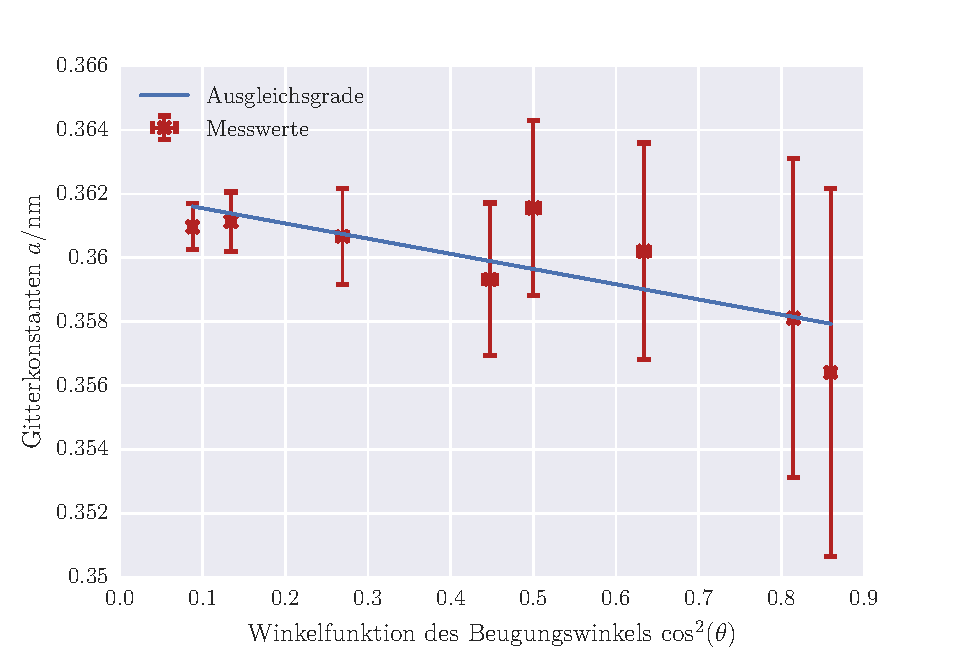
\includegraphics[scale=0.8]{../Grafiken/Gitterkonstante_Probe.pdf}
 \caption{Grafische Darstellung der berechneten Gitterkonstanten der untersuchten Probe mit linearer Regression.\label{fig:gitterkonstante_probe}}
 \end{figure} 
\FloatBarrier

\begin{figure}[!h]
 \centering
 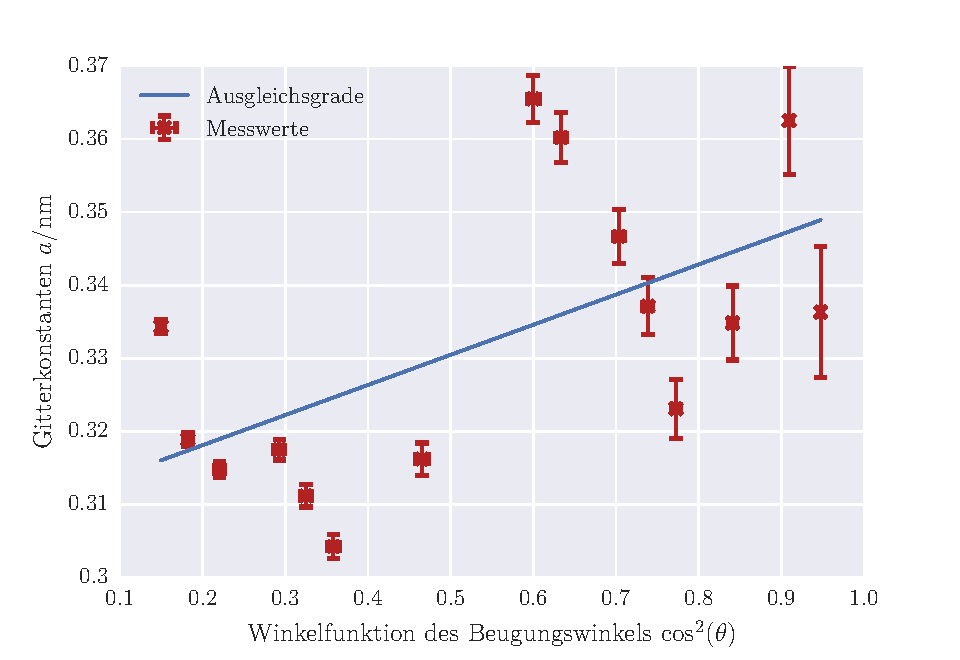
\includegraphics[scale=0.8]{../Grafiken/Gitterkonstante_Salz.pdf}
 \caption{Grafische Darstellung der berechneten Gitterkonstanten des untersuchten Salzes mit linearer Regression. \label{fig:gitterkonstante_salz}}
 \end{figure} 
\FloatBarrier
